The \textbf{Newton-Raphson method} (also known as Newton's method) is a way to quickly find a good approximation for the root of a real-valued function $f(x) = 0$ It uses the idea that a continuous and differentiable function can be approximated by a straight line tangent to it.
\subsection{How it Works ?}
Suppose you need to find the root of a continuous, differentiable function f(x)f(x), and you know the root you are looking for is near the point $x = x_0x=x 
0$. Then Newton's method tells us that a better approximation for the root is
\begin{equation}
 x_{1}=x_{0}-\frac{f\left(x_{0}\right)}{f^{\prime}\left(x_{0}\right)} 
\end{equation}
This process may be repeated as many times as necessary to get the desired accuracy. In general, for any $x$-value $x_n$ , the next value is given by
\begin{equation}
 x_{n+1}=x_{n}-\frac{f\left(x_{n}\right)}{f^{\prime}\left(x_{n}\right)} 
\end{equation}
\subsection{Geometric Representation}
Figure \ref{fig:nr1} is the picture to demonstrate what Newton's method actually does:
\begin{figure}[H]
    \centering
    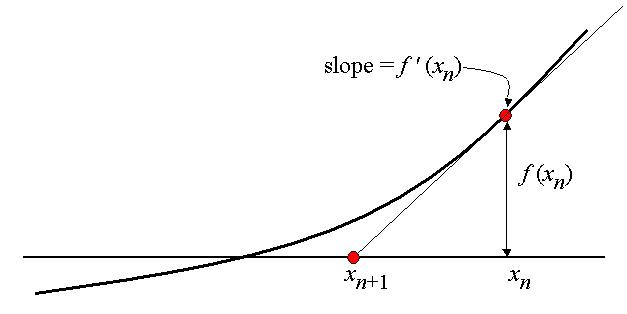
\includegraphics[scale=0.5]{Figures/Chapter2/newtonraphson1.png}
    \caption{Geometric Representation for \textbf{Newton-Raphson} method}
    \label{fig:nr1}
\end{figure}
We draw a tangent line to the graph of $f(x)$ at the point $x = x_n$. This line has slope $f'(x_n) $ and goes through the point $\big(x_n, f(x_n)\big)$
 Therefore it has the equation $y = f'(x_n)(x - x_n) + f(x_n)$. Now, we find the root of this tangent line by setting $y = 0$ and $x=x_{n+1}$ for our new approximation. Solving this equation gives us our new approximation, which is
 $
 x_{n+1}=x_{n}-\frac{f\left(x_{n}\right)}{f^{\prime}\left(x_{n}\right)} 
$
\subsection{Example With Matlab Code}
\label{Example2}
\vspace{0.38cm} \textit{Example: Find the root of the equation $x^2 - 4x - 7 = 0 $ near $x = 5$ to the nearest thousandth.}

We have our $x_0 = 5 $. In order to use Newton's method, we also need to know the derivative of ff. In this case, $f(x) = x^2 - 4x - 7$, and $f'(x) = 2x - 4$

Using Newton's method, we get the following sequence of approximations:
\begin{equation*}
    \begin{gathered}
{x_1} = 5 - \frac{{{5^2} - 4 \times 5 - 7}}{{2 \times 5 - 4}} = 5 - \left( {\frac{{ - 2}}{6}} \right) = \frac{{16}}{3} \approx 5.33333\\
{x_2} = \frac{{16}}{3} - \frac{{{{\left( {\frac{{16}}{3}} \right)}^2} - 4\left( {\frac{{16}}{3}} \right) - 7}}{{2\left( {\frac{{16}}{3}} \right) - 4}} = \frac{{16}}{3} - \frac{{\frac{1}{9}}}{{\frac{{20}}{3}}} = \frac{{16}}{3} - \frac{1}{{60}} = \frac{{319}}{{60}} \approx 5.31667\\
{x_3} = \frac{{319}}{{60}} - \frac{{{{\left( {\frac{{319}}{{60}}} \right)}^2} - 4\left( {\frac{{319}}{{60}}} \right) - 7}}{{2\left( {\frac{{319}}{{60}}} \right) - 4}} = \frac{{319}}{{60}} - \frac{{\frac{1}{{3600}}}}{{\frac{{398}}{{60}}}} \approx 5.31662.\\
{x_4} = 5.31662 - \frac{{{{(5.3362)}^2} - 4(5.3362) - 7}}{{2(5.3362) - 4}} = 5.31662
\end{gathered}
\end{equation*}

Code Matlab base on Newton-Raphson method:
\begin{lstlisting}
function [result,m]=NewtonRaphsonVsCount(x,f,range,n,x0)
%% input la bien so x, ham so f,range, so buoc lap n,x0 (neu co)
%output [result,m,]
%% giai thuat
df=diff(f,x,1);
ddf=diff(f,x,2);
newton= x-f/df;
%% Tim dieu kien bat dau bat fourier 
if exist('x0') == 0
    fourier=double(subs(f*ddf,x,range))
    for i =1:length(range)
        if fourier(i)>=0
            x0=range(i)
        end                             
    end
end
%% tim m de tinh sai so 
m=double(min(subs(abs(df), x, range)));
%% Bat dau giai thuat newton Raphson
X=[x0];
DeltaX=[0];
for i=1:n
    x_n=double(subs(newton,x,X(end)));
    X=[X;x_n];
    DeltaX=[DeltaX ; double(subs(abs(f)/m,x,x_n))];
end
n=[0:n]';
result=table(n,X,DeltaX);

\end{lstlisting}

We build solution for this example base on this function:
\begin{lstlisting}
syms x
range =[4 6];
f=x^2-4*x-7;
x0=5;
n=4;
[result]=NewtonRaphsonVsCount(x,f,range,n,x0);
disp(result)
\end{lstlisting}

\begin{figure}[H]
    \centering
    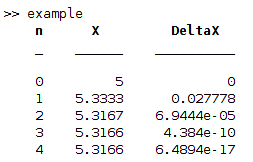
\includegraphics{Figures/Chapter2/resultNewton.png}
    \caption{Result for section \ref{Example2} in Matlab}
    \label{fig:Piecewise}
\end{figure}

\subsection{Limitations of Newton's Method}


Newton's method may not work if there are points of inflection, local maxima or minima around $x_0$  or the root.

For example, suppose you need to find the root of $27x^3 - 3x + 1 = 0$ which is near $x = 0$.
The correct answer is $-0.44157265\ldots$ However, Newton's method will give you the following:

\begin{equation*}
     x_{1}=\frac{1}{3}, x_{2}=\frac{1}{6}, x_{3}=1, x_{4}=0.679, x_{5}=0.463, x_{6}=0.3035, x_{7}=0.114, x_{8}=0.473, \ldots 
\end{equation*}

This is very clearly not helpful. That's because the graph of the function around $x = 0$ looks like in figure \ref{fig:limitNewton}.
\begin{figure}[H]
    \centering
    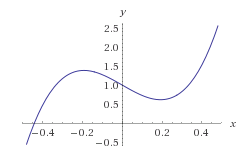
\includegraphics{Figures/Chapter2/limitNewton.png}
    \caption{Example the limit of \textsc{Newton-Raphson} Method }
    \label{fig:limitNewton}
\end{figure}
As you can see, this graph has a local maximum, a local minimum and a point of inflection around $x = 0$. To see why Newton's method isn't helpful here, imagine choosing a point at random between $x = -0.19$ and $x=0.19$ and drawing a tangent line to the function at that point. That tangent line will have a negative slope, and therefore will intersect the $y$-axis at a point that is farther away from the root. So this method doesn't always give the expected result.
\subsection{Significance of Newton-Raphson in Mechanical Solution }
Consider the following system of nonlinear equations:
\begin{equation}
\label{eqn:26}
    P(u)=f
\end{equation}
where $u = [u_1, u_2,\ldots,u^n]^T$ is a vector of unknowns, $f=4 [f_1, f_2,\ldots , f_n]^T$ is a vector of known quantities, and $P(u)= [P_1(u), P_2(u),\ldots, P_n(u)]^T$ is a vector of nonlinear
functions of $u$. In structural applications, $u$ is often the displacement vector, $f$ is the
applied force vector, and $P(u)$ is the internal force vector. Thus, Eq. (\ref{eqn:26}) is the
equilibrium between internal and applied forces. In the linear problems 
the internal force vector is a linear function of u such that $P(u)=K.u$ with $K$ being
a constant stiffness matrix. Then, solving a system of linear equations is equivalent
to calculating the inverse matrix of K and multiplying it with the vector,
$f$. 

Since P(u) is a nonlinear function of $u$, nonlinear analysis focuses on how to solve Eq. (\ref{eqn:26}) accurately and effectively. The solution methods applicable to general nonlinear functions are all iterative. Starting from an initial estimate, $u_0$, the increment, $\Delta u$, of the solution is obtained by solving a system of linear equations. Linearization is involved in this process. After obtaining the increment, the solution is iteratively updated until a specified convergence criterion is satisfied. Different methods are available according to the way to calculate the increment,
$\Delta u$; 

\textsc{Newton-Raphson} method is popular in numerical analysis to find the roots of nonlinear
equations. Basically, most numerical methods for solving a system of nonlinear
equations assume an initial estimate, u0, and find its increment, Δu, so that the
new estimate, $u_0 + \Delta u,$ is close to the solution to Eq. (\ref{eqn:26}). In order to find the increment, the nonlinear equations are locally approximated by linear ones. This process is repeated until the original nonlinear equations are satisfied. these will be discussed in section \ref{sec:nonlinear}.
